\documentclass[11pt, twoside]{article}

\usepackage{ucs}
\usepackage{graphicx}
\usepackage{verbatim}
\usepackage{anyfontsize}
\usepackage[T1]{fontenc}
\usepackage[utf8x]{inputenc} 
\usepackage[english, russian]{babel}
\usepackage{amssymb, amsfonts, amsmath, mathtext, cite, enumerate, float}
\usepackage{geometry}
\usepackage{fancyhdr}
\usepackage{epstopdf}
\fancypagestyle{titlestyle}
{
	\fancyhead{}
	\fancyfoot{}
	\renewcommand{\footrulewidth}{0.0 mm}
	\renewcommand{\headrulewidth}{0.0 mm}
}

\geometry{left=2cm}
\geometry{right=1.5cm}
\geometry{top=2cm}
\geometry{bottom=2cm} 

\newcommand\measurepage{\dimexpr\pagegoal-\pagetotal-\baselineskip\relax}

\newcommand\fillpage{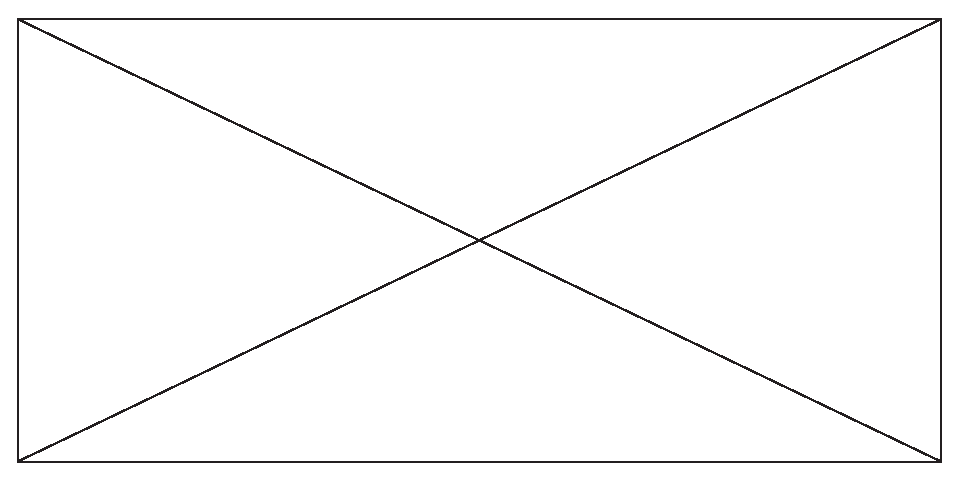
\includegraphics[width=\textwidth, height=\measurepage]{img/fill_page.eps} \newpage}

\newenvironment{itemize*}%
{\begin{itemize}%
		\setlength{\itemsep}{1pt}%
		\setlength{\parskip}{1pt}}%
	{\end{itemize}}


\newenvironment{enumerate*}%
{\begin{enumerate} %
		\setlength{\itemsep}{1pt}%
		\setlength{\parskip}{1pt}}%
	{\end{enumerate}}

\newcounter{number_of_meeting}\setcounter{number_of_meeting}{0}

\renewcommand{\labelenumii}{\arabic{enumi}.\arabic{enumii}.}
\renewcommand{\labelenumiii}{\arabic{enumi}.\arabic{enumii}.\arabic{enumiii}.}
\renewcommand{\labelenumiv}{\arabic{enumi}.\arabic{enumii}.\arabic{enumiii}.\arabic{enumiv}.}
\pagestyle{fancy}
{
\fancyhead{}
\fancyhead[C]{PML30 Saint-Petersburg}
\fancyfoot{}
\fancyfoot[LE,RO]{\thepage}
\fancyfoot[C]{Russia, St. Petersburg, Physics-Mathematics Lyceum №30. 2014-2015}
}


\begin{document}

	
	%\thispagestyle{titlestyle}
\begin{titlepage}
	
	\begin{center}
		\LARGE\textit{Center for robotics \\ Physics-Mathematics Lyceum 30}
        \begin{figure}[H]
         	\center{
	            
\includegraphics[scale=0.45]{days/Title/images/01}  
				
\includegraphics[scale=0.15]{days/Title/images/02}
			}
        \end{figure}
		\vspace{3em}
		
		\LARGE{Engineering book of \\ Competition First FTC}
		
		\vspace{2em}
		
		\bf\fontsize{50}{60}\selectfont Team PML30-${\varphi}$ \\ 9746 \fontsize{11}{13}\selectfont
			
	\vspace{6em}
		
		\begin{figure}[H]
			\center{
			    
\includegraphics[scale=0.12]{days/Title/images/03}  
		        
\includegraphics[scale=0.7]{days/Title/images/04}
		        
\includegraphics[scale=1.1]{days/Title/images/05}
		        
\includegraphics[scale=0.3]{days/Title/images/06}
			}
		\end{figure}
			
		\LARGE\normalfont Saint-Petersburg, Russia	\\ 2015
	\end{center}
\end{titlepage}

\newpage

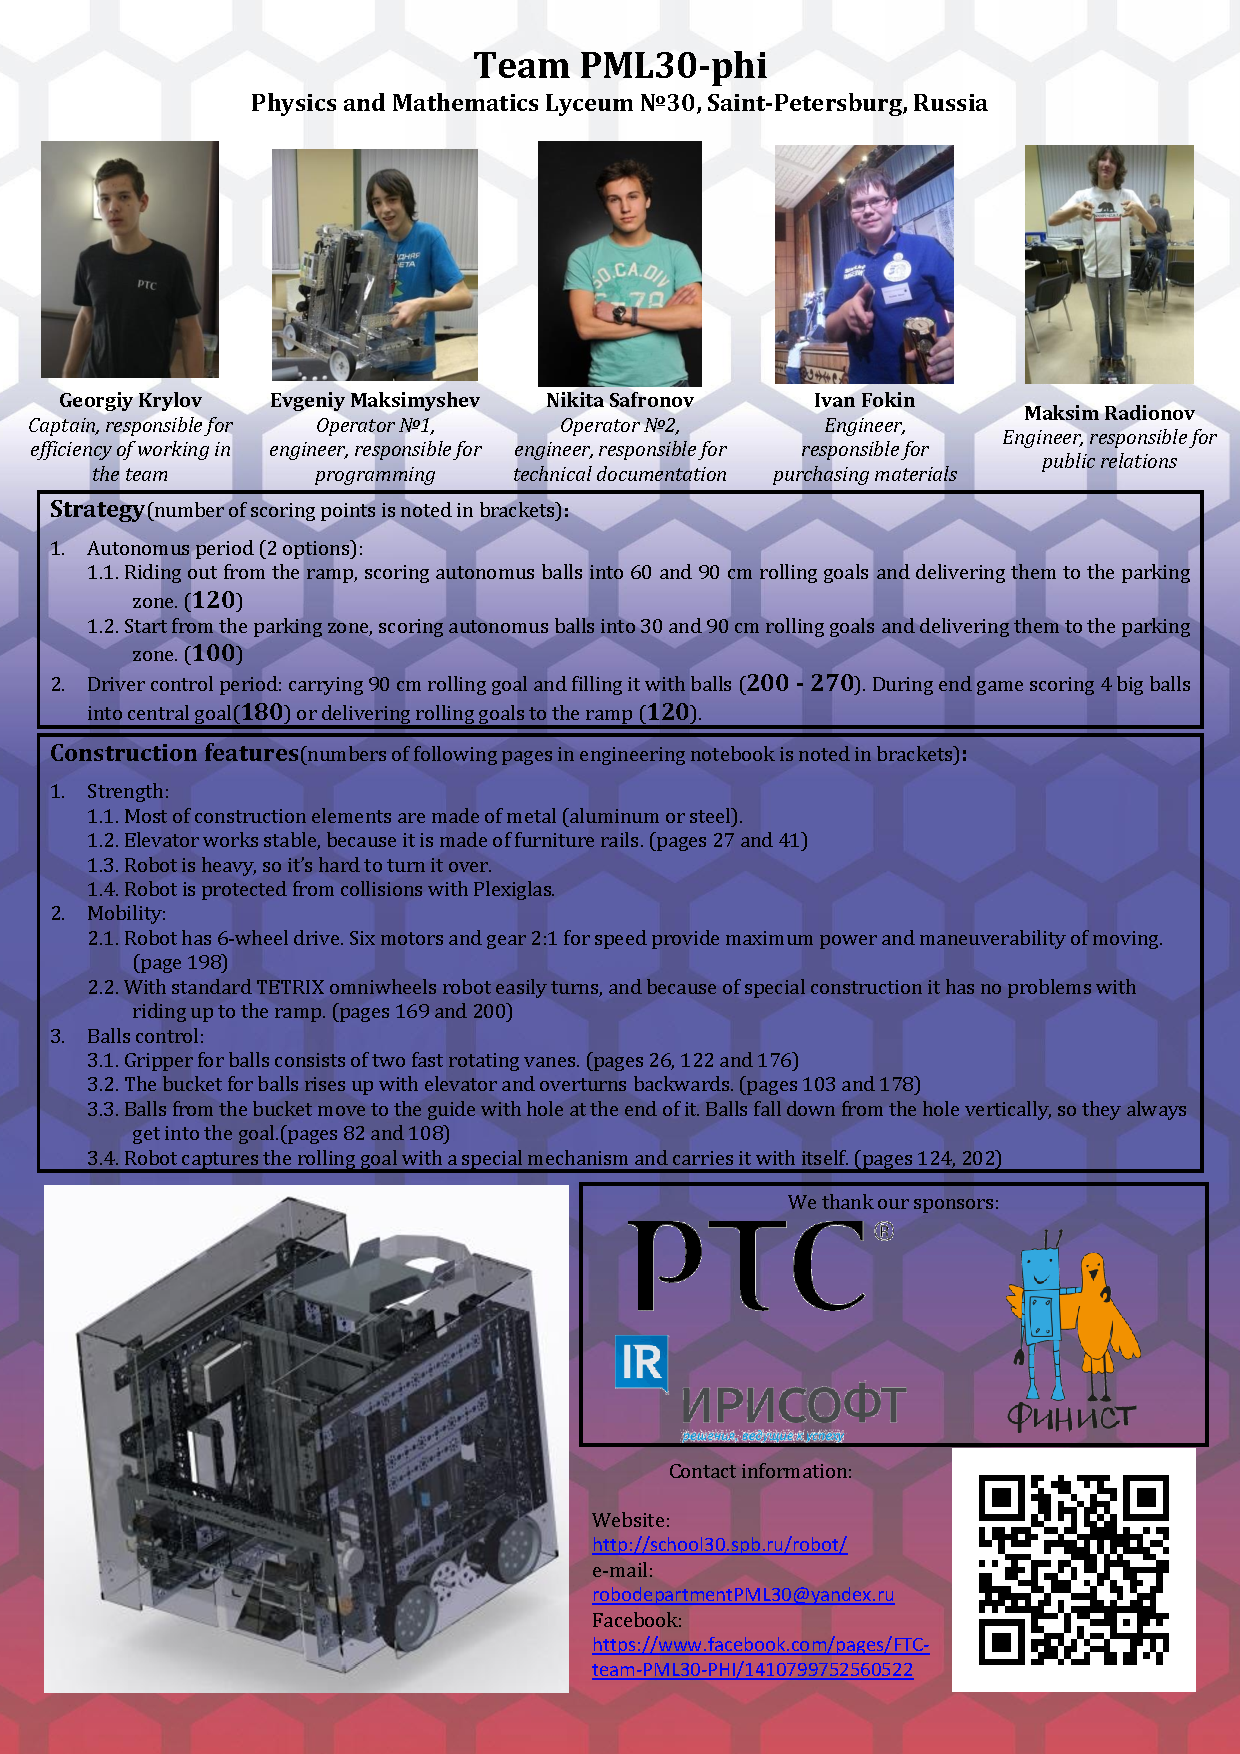
\includegraphics[scale=0.8]{days/Title/images/PML30-PHI-infolist_judge}


	
	%\tableofcontents{}
	%\newpage
	
	%
\section{Team PML 30 ${\varphi}$} 
	Team PML 30 ${\varphi}$ was assembled in September 2014 in the Russian city of St. Petersburg from 3 novices and 2 participants with experience. Tasks and roles were distributed among the participants, and we established safety rules. In the first place the team put spreading principles of gracious professionalism to others. All decisions were made collectively inside team with discussion to find the most optimal solutions. 
	During the year we took part in many events and everywhere we have tried to attract attention to our team and encourage people to take part in FTC. Also we pursued and distributed the principles of honorable professionalism. Talking to the press, we hoped to attract more attention to our team and to the competition in general, as well as attracting sponsors. The latter was important because of the need for funds - purchasing materials and equipment costs a lot.
	The team took part in the three qualifying competitions and in the regional finals. In all of them we made new contacts, shared experience and provided mutual assistance to other teams. In the first qualifying rounds in Sochi we met Stuy Fission 310 from USA and maintain contact with them to this day. On regional finals, we met with a team from Romania, Auto Vortex, and keep in touch with them through Facebook. Also, there is an active group chat with a large number of Russian teams. You can find the team page in Facebook at the address https://www.facebook.com/pages/FTC-team-PML30-PHI.
	To increase the efficiency of our team work we used the version control system GitHub, which allows the entire team to work simultaneously on a single projects without losing files and providing easy way to resolve roblems. Also for writing technical books we been used professional typesetting system LaTeX.
	\begin{figure}[H]
		\center{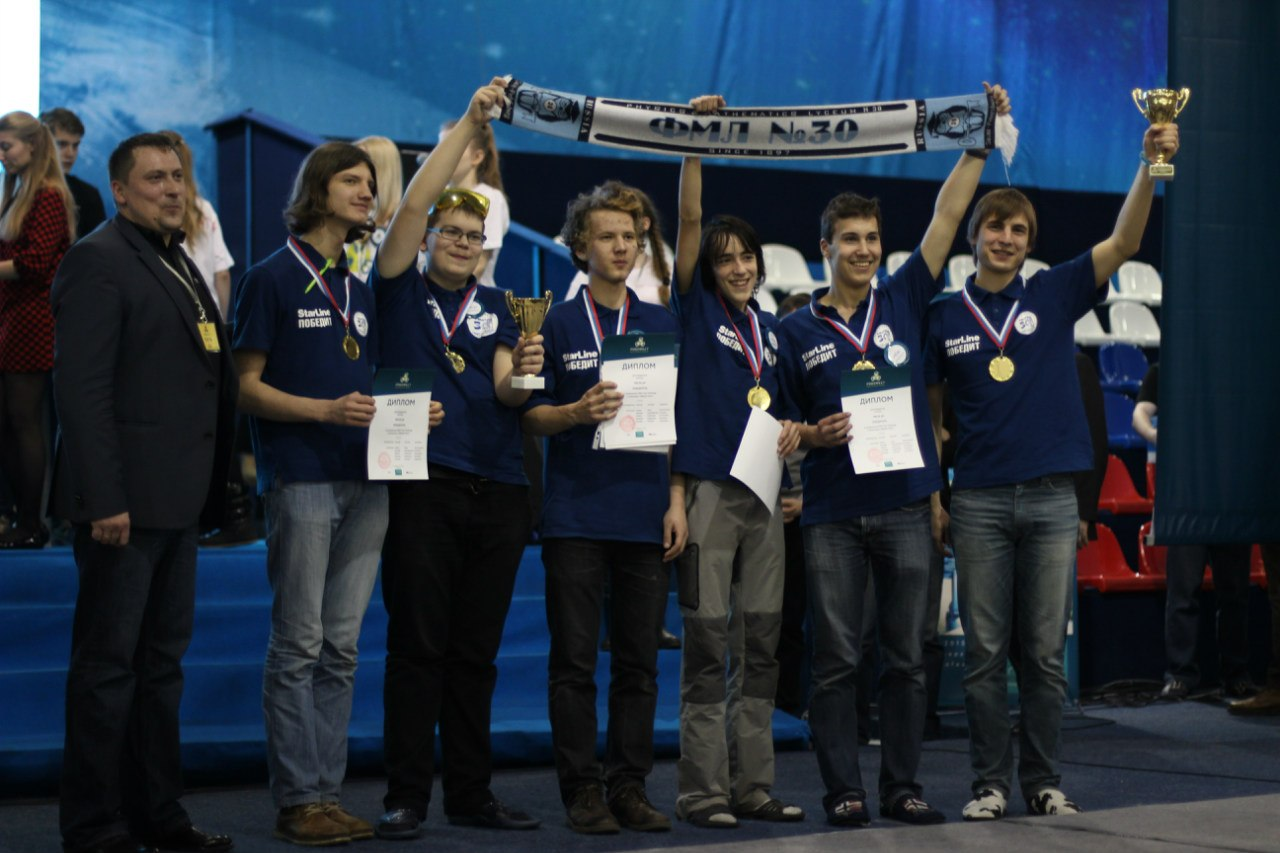
\includegraphics[scale=0.2]{days/Team/images/09}}\\
	\end{figure}[H]
\fillpage

\subsubsection{Instructors}:

\begin{figure}[H]
	
	\begin{minipage}[h]{0.47\linewidth}
		Luzin Dmitry\\
		\emph{Head of Robotics Department in Phys-Math Lyceum 30, Saint-Peterburg, Russia. Main coach of FTC team.\\}
		\emph{Information: 25 years old, in robotics 5 years, in FTC 3 years.}
	\end{minipage}
	\hfill
	\begin{minipage}{0.47\linewidth}
		\center{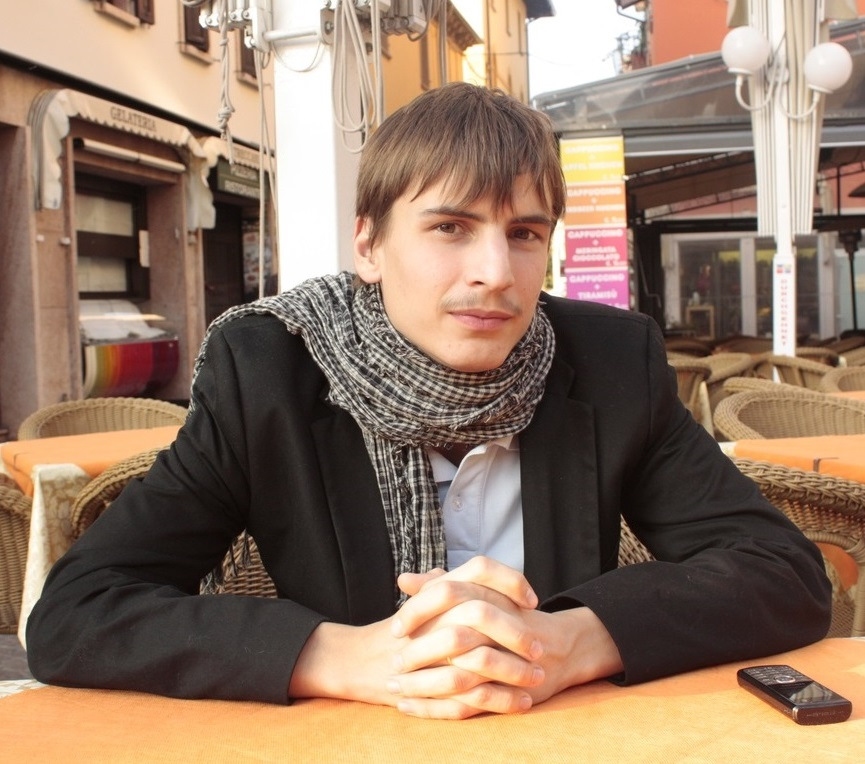
\includegraphics[scale=0.3]{days/Team/images/07}}\\
	\end{minipage}
	\vfill
	\begin{minipage}[h]{0.47\linewidth}
		\center{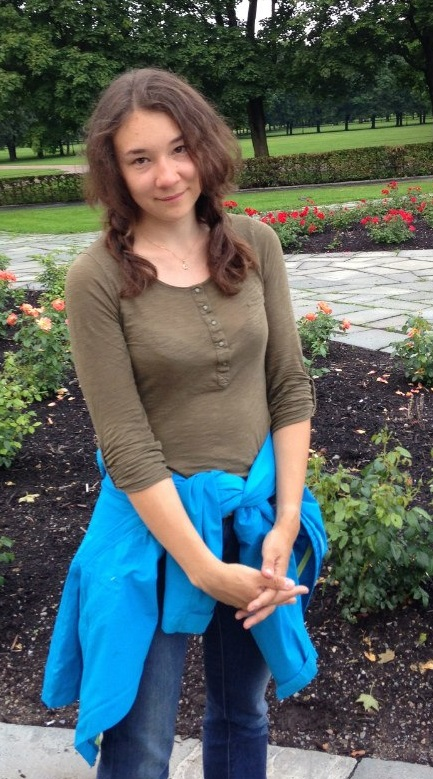
\includegraphics[scale=0.35]{days/Team/images/08}}\\
	\end{minipage}
	\hfill
	\begin{minipage}{0.47\linewidth}
		Luzina Ekaterina \\
		\emph{Professor of Robotics Department in Phys-Math Lyceum 30, Saint-Peterburg, Russia. Tutor of FTC team. \\}
		\emph{Information: 25 years old, in robotics 5 years, in FTC 3 years.}
	\end{minipage}
\end{figure}

\begin{figure}[H]
	\begin{minipage}[h]{0.47\linewidth}
		\center{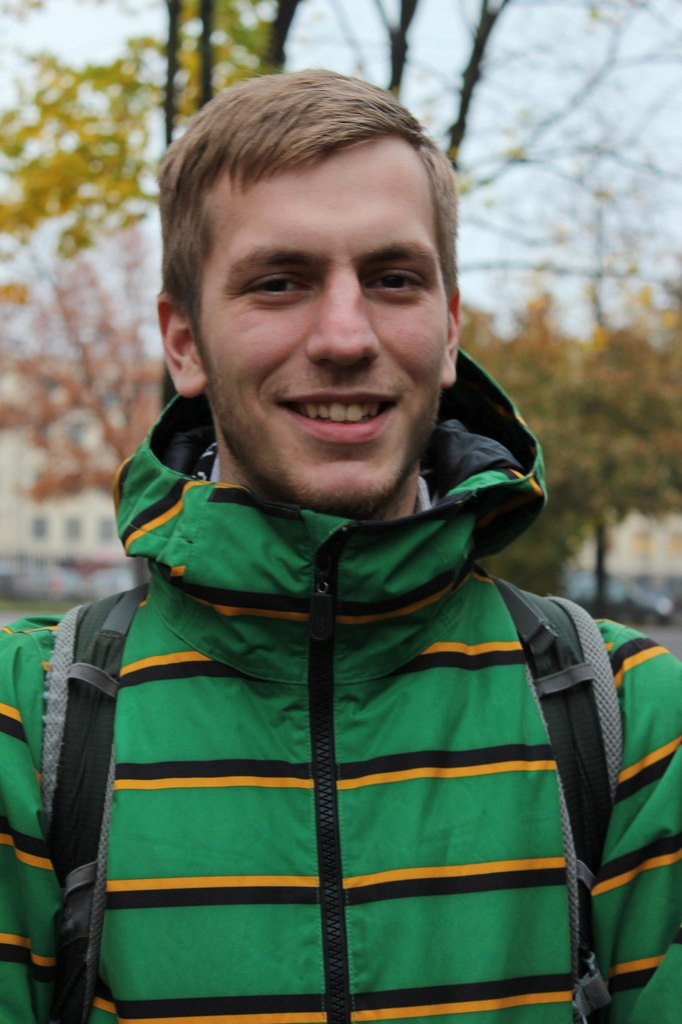
\includegraphics[scale=0.25]{days/Team/images/05}}\\
	\end{minipage}
	\hfill
	\begin{minipage}{0.47\linewidth}
		Fedotov Anton \\ 
		\emph{Professor of Robotics Department in Phys-Math Lyceum 30, Saint-Peterburg, Russia. Tutor of FTC team. \\}
		\emph{Information: 22 years old, in robotics 4 years, in FTC 3 years.}
	\end{minipage}	
	\vfill 
\end{figure}

\fillpage

\subsubsection{Team members}
\begin{figure}[H]
	\begin{minipage}[h]{0.47\linewidth}
		\center{
\includegraphics[scale=0.08]{days/Team/images/06}}		
	\end{minipage}
	\hfill
	\begin{minipage}[h]{0.47\linewidth}
		Krylov Georgii \\
		\emph{Role in team: captain, coordinator of the action operators in game, responsible for the modification of robot.\\}
		\emph{Information: 17 years old, in robotics 3 years, in FTC 3 years. \\}
		\emph{Why I chose FTC: "I chose the FTC, because I like to come up with the design of robots and turn their ideas into reality, because every time I feel the Creator, who created a new creature."}		
	\end{minipage}
	\vfill 
	\begin{minipage}[h]{0.47\linewidth}
		Radionov Maxim\\
		\emph{Role in team: communication with the team and community, decorating robot, Power Design, reserve operator. \\  }
		\emph{Information: 16 years old, in robotics 3 years, in FTC 1 year. \\}
		\emph{Why I chose FTC: "Because I like to create a robot from scratch, from somethink, I can do with my hands: cut, drill and assemble."}					
	\end{minipage}
	\hfill
	\begin{minipage}[h]{0.47\linewidth}
		\center{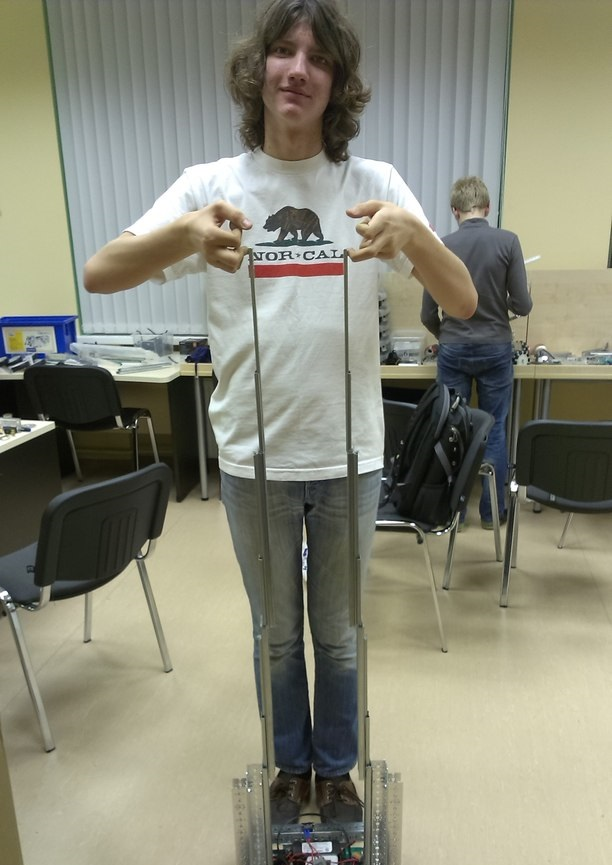
\includegraphics[scale=0.25]{days/Team/images/02}}\\
	\end{minipage}
	\vfill
	\begin{minipage}{0.47\linewidth}
		\center{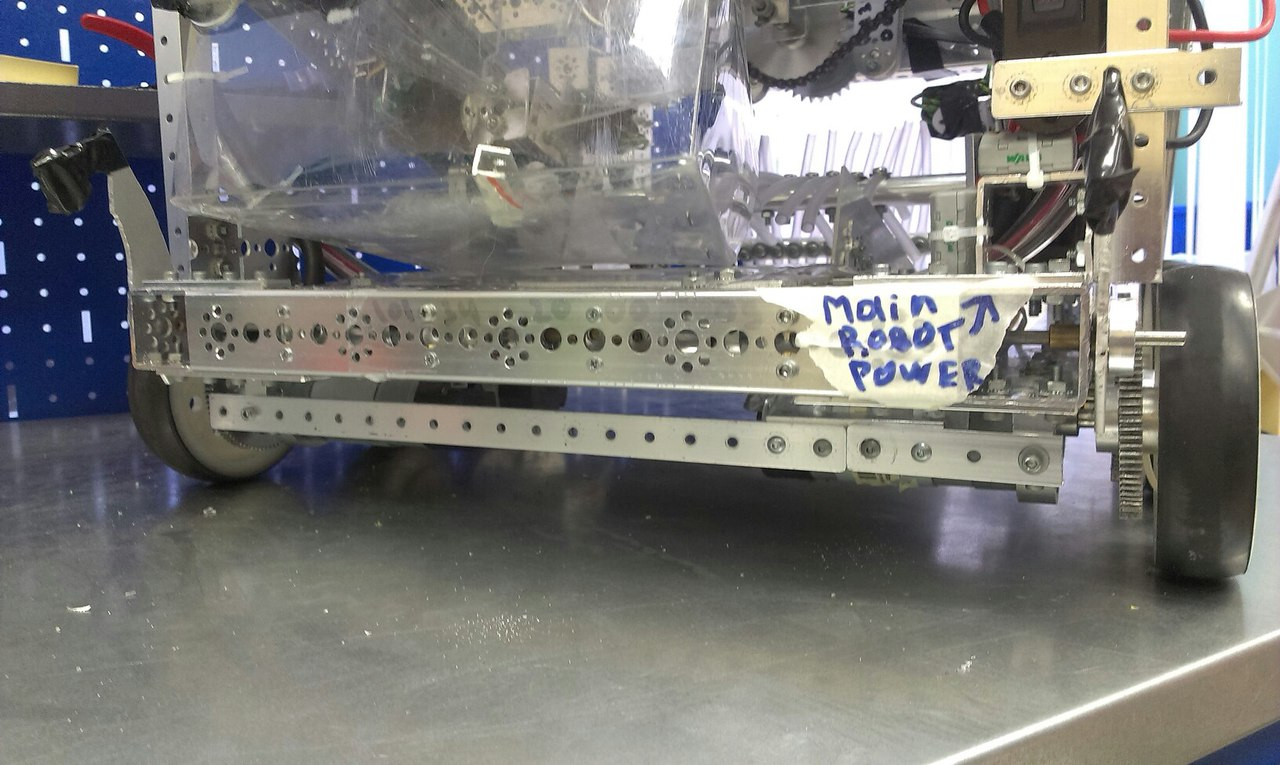
\includegraphics[scale=0.22]{days/Team/images/03}}\\
	\end{minipage}
	\hfill
	\begin{minipage}{0.47\linewidth}
		Safronov Nikita\\
		\emph{Role in team: manipulator-1,  creation of 3D models, chief engineer, responsible for the assembly robot.\\}
		\emph{Information: 16 years old, in robotics 3 years, in FTC 1 years.\\} 
		\emph{Why I chose FTC: "I have chosen FIRST because I enjoy working with mechanisms and finding unusual technical decisions for solving problems. Also working on this project helps me to get new skills in a sphere of engineering. In this case I know, that I don,t spend my time in vain."}				
	\end{minipage}
\end{figure}

\begin{figure}[H]
	\begin{minipage}{0.47\linewidth}
		Maksimychev Evgeny\\
		\emph{Role in team: manipulator-2, responsible for the technic of safety, responsible for the writting of technical book. \\}
		\emph{Information: 15 years old, in robotics 2 years, in FTC 1 year. \\}
		\emph{Why I chose FTC: "This is an interesting project that allows to implement some innovative solutions. In addition to the skills of designing robots, we also obtain the skills of the technical documentation and communication with colleagues which makes this competition as close to real engineering problems."}			
	\end{minipage}
	\hfill
	\begin{minipage}{0.47\linewidth}
		\center{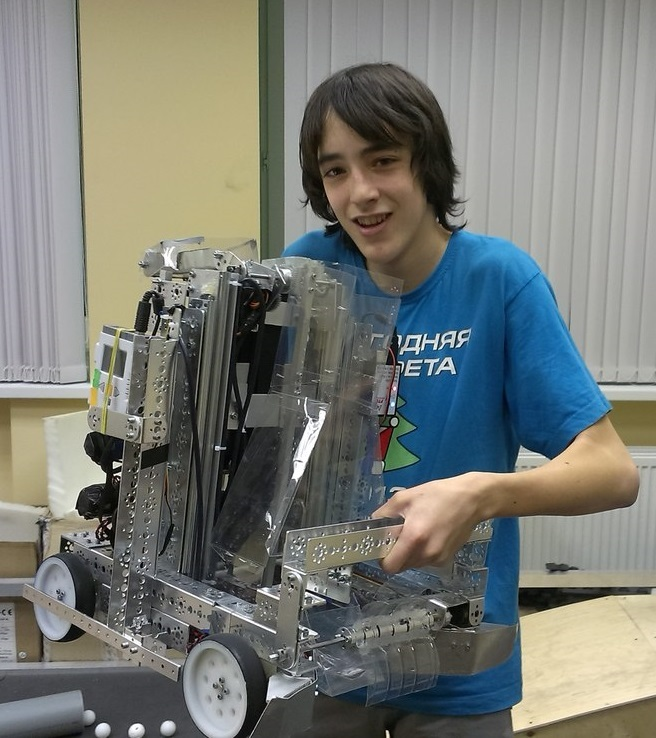
\includegraphics[scale=0.25]{days/Team/images/04}}\\
	\end{minipage}
	\vfill	
	\begin{minipage}{0.47\linewidth}
		\center{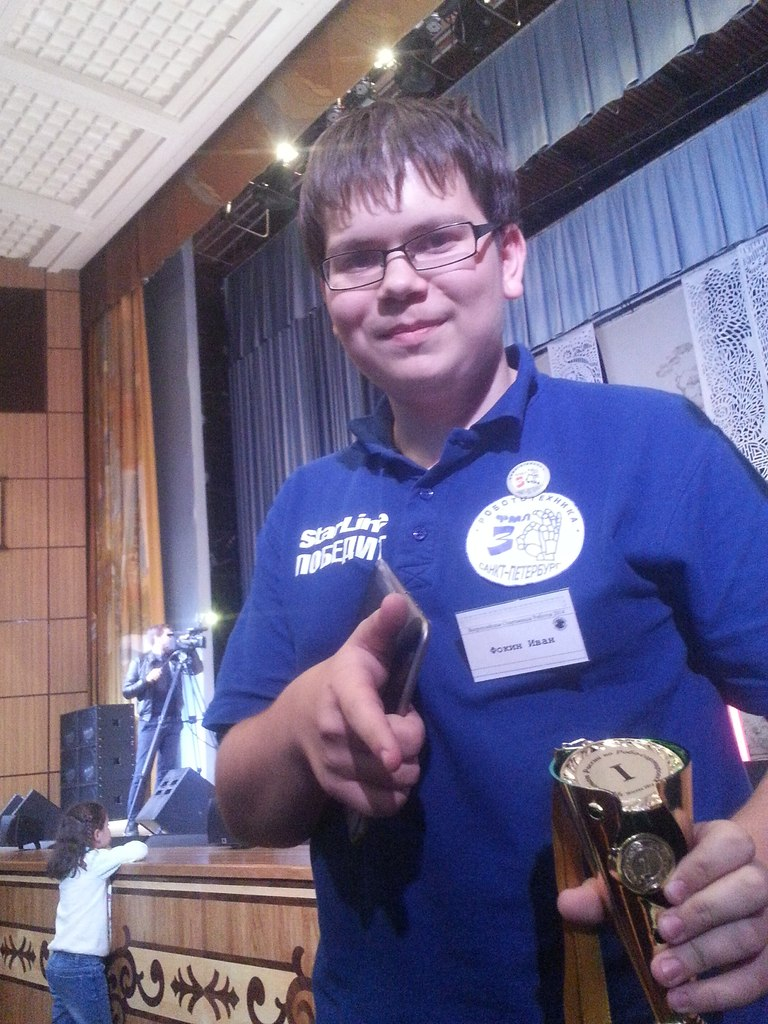
\includegraphics[scale=0.2]{days/Team/images/01}}			
	\end{minipage}
	\hfill
	\begin{minipage}{0.47\linewidth}
		Fokin Ivan\\
		\emph{Role in team: purchase of materials,  development strategy in the game,  communication with the press, reserve  manipulator.\\ }
		\emph{Information: 17 years old, in robotics 5 years, in FTC 3 years. \\ } 
		\emph{Why I chose FTC:" When I first I attended the event FTC saw hefty metal robots, with enthusiasm and without hesitation decided that I would like to do this."}		
	\end{minipage}	
\end{figure}

\fillpage



	%\section{Events}
	\subsubsection{Qualifying competitions}
		\begin{enumerate}
			\item Sochi. 21-23.11.2014. 
			Sochi was the first time the team participated in a comptetition. There, our team felt the spirit of FTC comptetion and noble professionalism for the first time. We got work experience all day and all night, began to make acquaintance among the teams, and providing all possible help we could. The planning and organization were all very nice. The most memorable contact we made was with the American team Stuy Fission 310, with which we now keep in touch. As a result we won a Think Award and a pass to the Regional final.
			\begin{figure}[H]
				\center{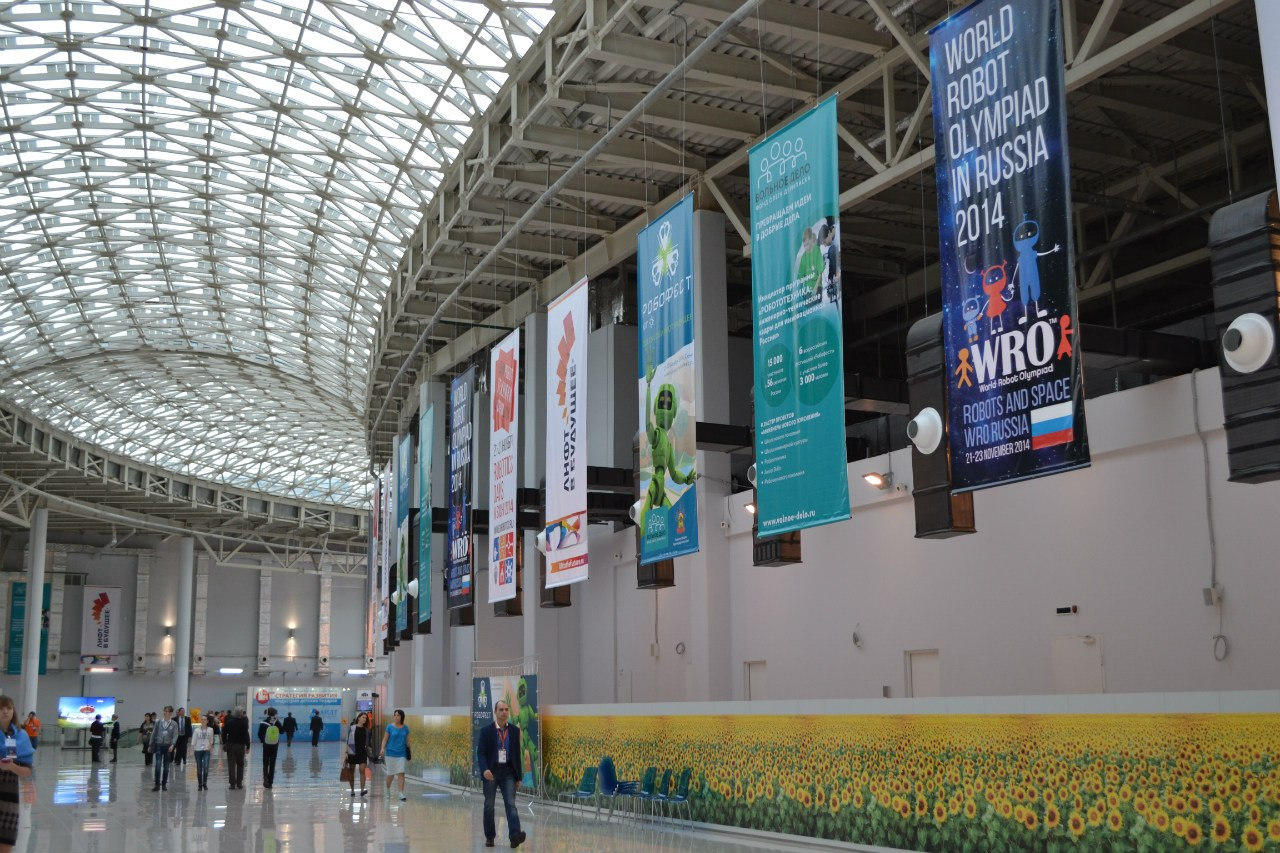
\includegraphics[scale=0.25]{days/Events/images/6}}
			\end{figure}
			\item Ryazan. 13-14.12.2014. 
			Our first priority was to train on a real field. These competitions were quite small and quiet, all the teams communicated abundantly and shared ideas freely. We all felt comfortable there. The team helped to assemble and disassemble the field. As a result - Winner Alliance Award and Think Award. 
			\begin{figure}[H]
				\center{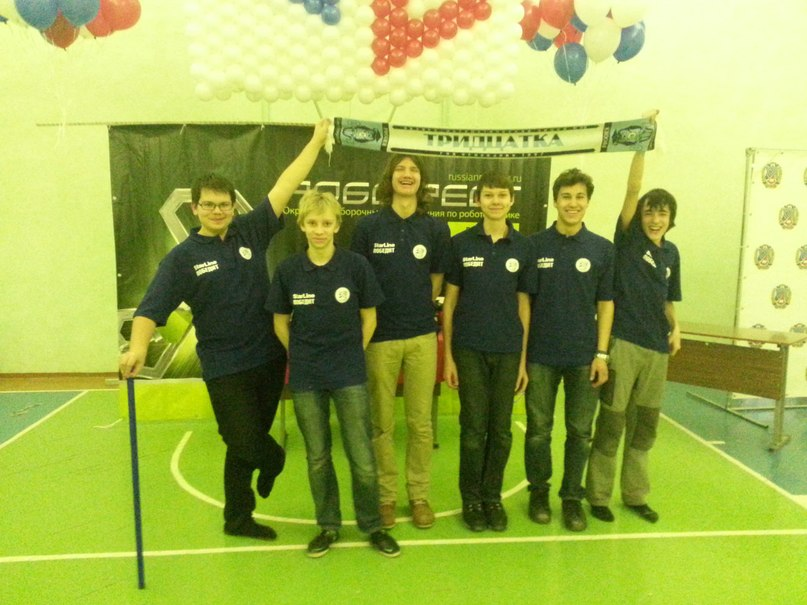
\includegraphics[scale=0.4]{days/Events/images/1}}
	     	\end{figure}	
			\item Perm. 27-29.01.2015. 
			Dress rehearsal before the regional final. It was great organized event where we were able to practice all aspects of the competition. Including such important skills as the choice of Composes alliances finale. Also we strongly helped to organized technical part. As a result - the Winner Alliance Award and Inspire Award.
			\begin{figure}[H]
				\center{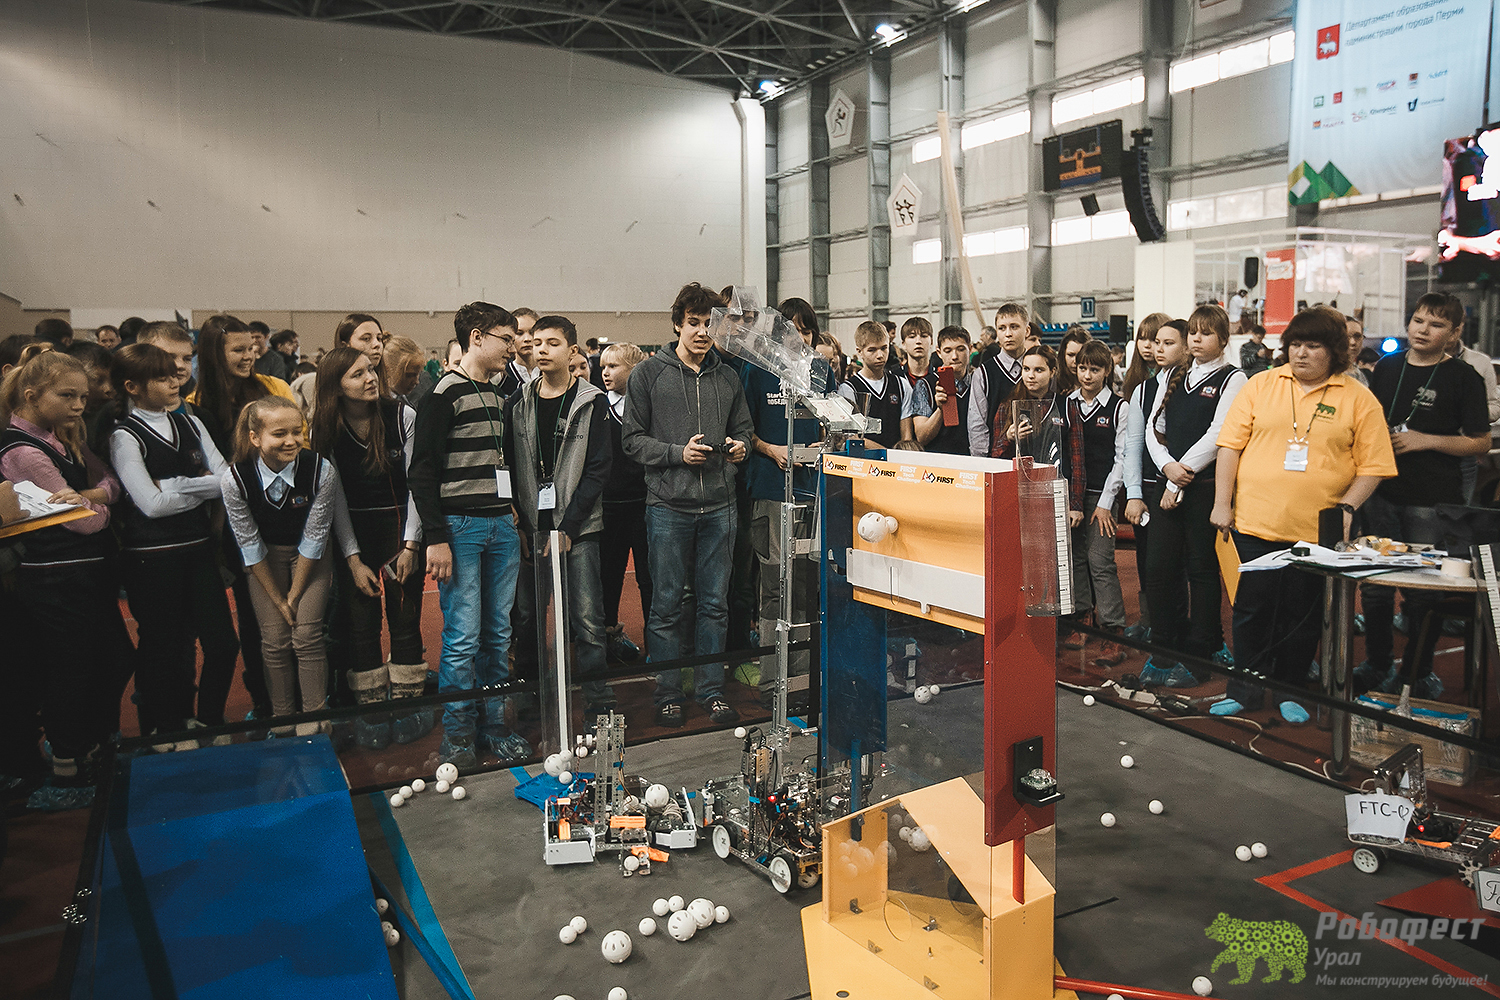
\includegraphics[scale=0.22]{days/Events/images/3}}\\
	     	\end{figure}
		\end{enumerate}  
	\subsubsection{Regional final. 11-13.02.2015}	
	This was the event, to which the team had been preparing for for six months. Approaching the competition with fully finished. At competitions communicated with all the teams that were there, discussing strategy and offering their help. During the competition statistics were conducted on all the teams. It helped in choosing allies for the final. Was also had an action plan for an alliance with any team. In the final, having received a the choice of allies, we chose the team with the most stable results, and the bet was at collaborative interaction of any pair of robots. Results: Winner Alliance Award, Inspire Award and the pass to World Championship in Saint Louis.
	\begin{figure}[H]
		\center{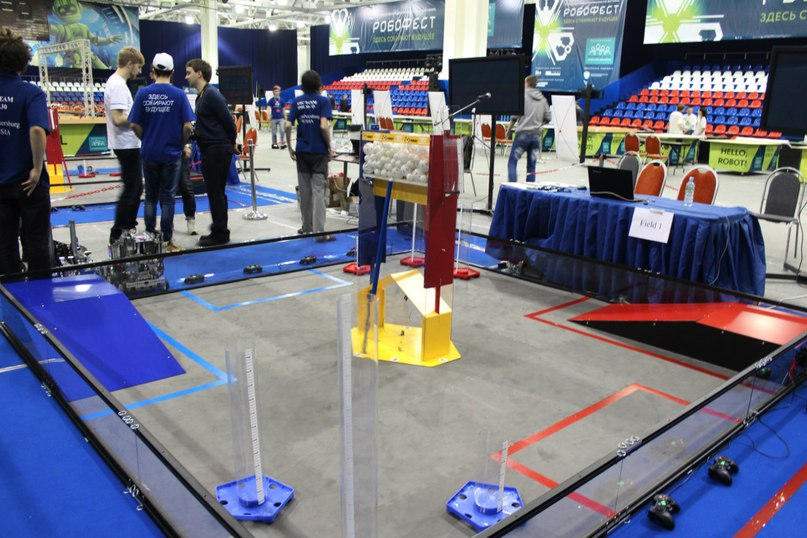
\includegraphics[scale=0.45]{days/Events/images/2}}\\
	\end{figure}
	\newpage			
	\subsubsection{CRDI RTC. 24.11.2014}
	Central Russian Institute of Robotics and Technical Cybernetics. A tour was organized for the team in the institute, where we could see the real processes of development of detailed design for robotics. There we saw several project summaries at different stages of development - from drawings to finished models, as well as commercially ready products. From there we learned some ways on how to organize. Internet adress http://www.rtc.ru.
	\begin{figure}[H]	
		\center{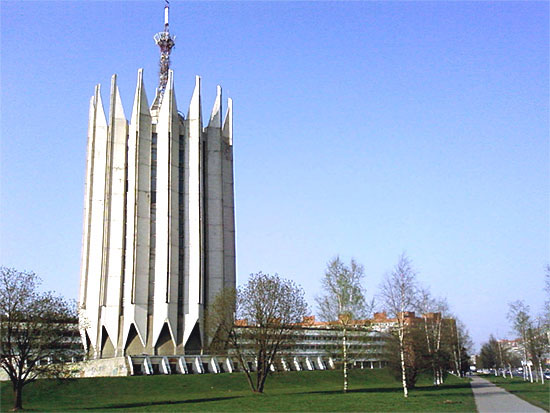
\includegraphics[scale=0.5]{days/Events/images/5}}\\
	\end{figure}
	\subsubsection{PML30 POLYGON. 08.02.2015}	
	PML30 POLYGON competitions are carried out by our organization. Their main  misrepresented that participant receives a rear and parts for its decision merely on the competition, compliance with the maximum being equal. We also demonstrated the FTC involving the participation.
	\begin{figure}[H]
		\center{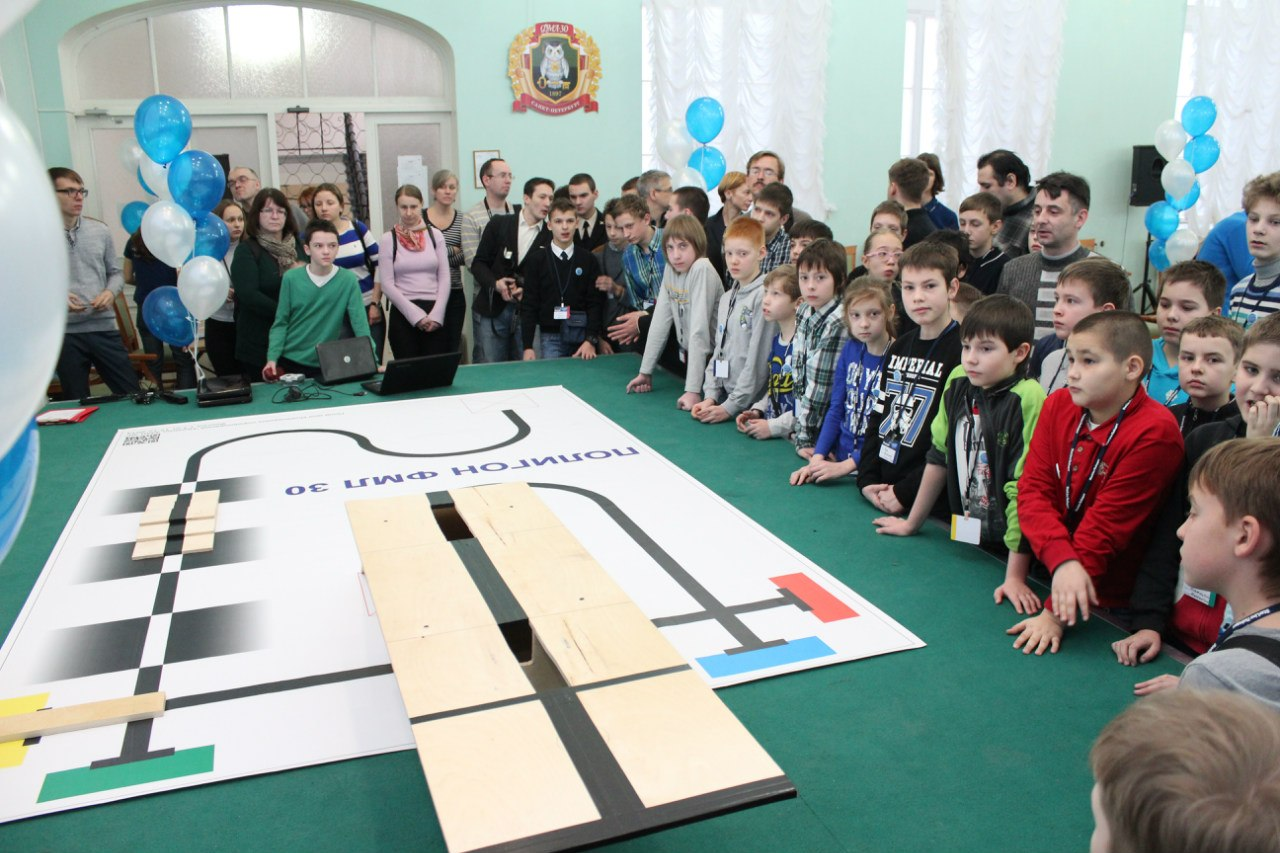
\includegraphics[scale=0.25]{days/Events/images/7}}\\
    \end{figure}
    \subsubsection{GeoScan. 10.03.2015}
	A Russian company thatproduces and sells unmanned aerial photography systems. There we were clearly shown how the office is designed, as well as the distribution of responsibilities and tasks, and what the internal interaction is like. Also, we were shown the whole production line. Internet adress http://geoscan.aero/.
    \begin{figure}[H]
    	\center{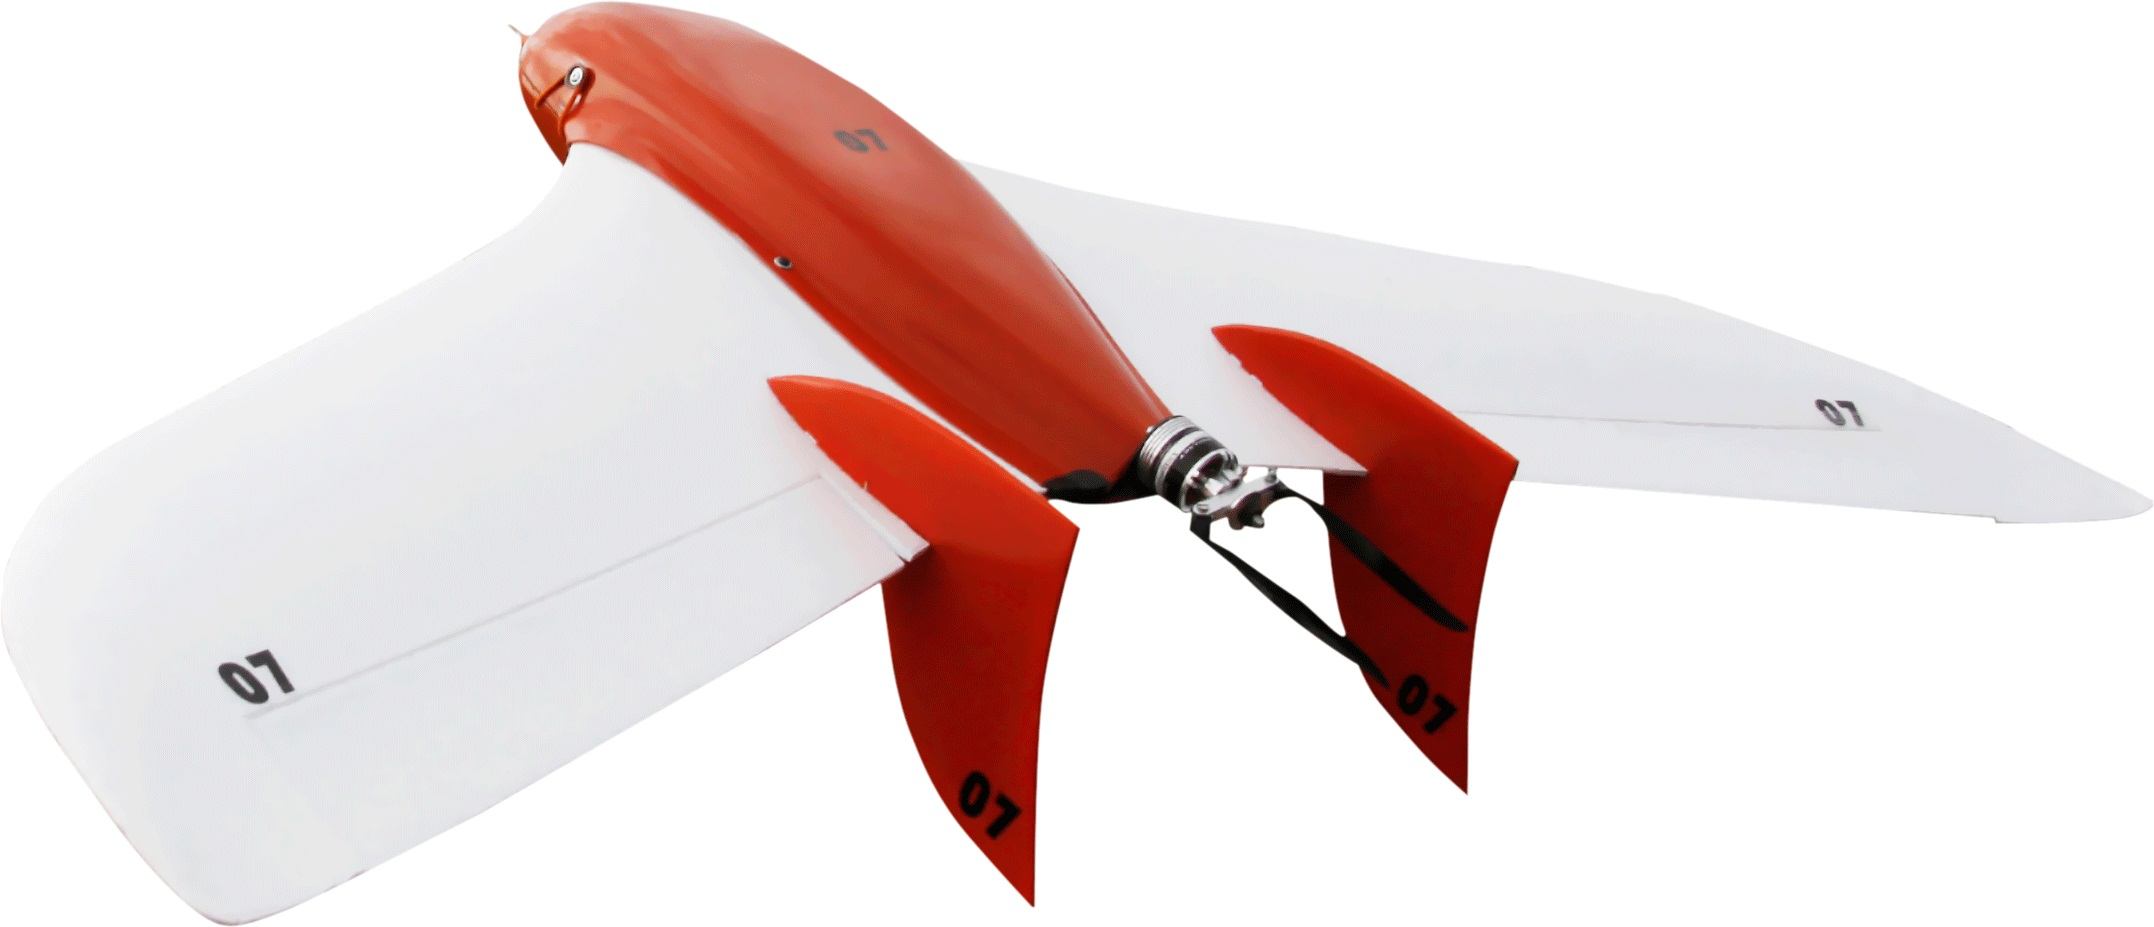
\includegraphics[scale=0.2]{days/Events/images/4}}\\	
    \end{figure}
	\subsubsection{PTC live Tech Forum. 24.03.2015}
	 The team was invited to participate in PTC Live Tech Forum. We will present the successfull path of 3D model creation in Creo Parametric, tell about important tips and show how CAD modelling helped us to build the robot.
	
	\subsubsection{Summer camp on Robotics}
	In the camp in 2015, team members will conduct a robotics engineering course based on constructor TETRIX, attracting more people to the FTC.
	
	\fillpage
		
		
		
		
		
		
		
		
		
	%\section{Business plan}
	\subsection{introduction}
	We take a responsible approach to finding sponsors. And also try to spend money effectively advance thinking through the details and equipment, finding ways to get them maximum benefit. Some sets we received as prizes in competitions.
	
	\subsection{Our sponsors and their support}
		\subsubsection{PTC and Irisoft}
		PTC and Irisoft representative in Russia is the one company that has helped us to begin to engage FTC. They provided us the first set of Tetrx within the program's Score Thehnic which involved our Lyceum. They provide us with a different command symbols plus small gifts for other teams. They help us with the delivery of details from U.S.A. We use them programa Creo for creating 3D models. We also take part in events organized by them.
		\subsubsection{Robofinist}	
		Robofinist Charitable Foundation organized by Temur Amindzhanov and by Starline. They offered us its assistance as an organization in our city with outstanding achievements. They help to financially each month to give us 2000 Dolars, parts and equipment.
		\subsubsection{Volnoe Delo}
		Volnoe Delo is one of the largest charitable foundations in Russia. It was established by Oleg Deripaska. We are participants of the program ROBOTOTEHNIKA.As support they sent us free game field.They also engaged in training teachers and judges, including our own.They engaged in the organization of competitions FTC in Russia and are sponsoring a trip this year's winners to St. Louis.	
		\subsubsection{Physics-Mathematics Lyceum №30}
		Physics-Mathematics Lyceum №30 is a school in which is our organization. It provides us with a comfortable space and material assistance, as well as leaders.
		
	\subsection{Purchase of materials.}
		\subsubsection{Our method}
		When we started robotics we had not a lot of money and we used only some basic materials. Now we found sponsors and firstly plan the details and equipment that we need to buy and then buy them.Such an approach allows us to find more effective solutions.
		\subsubsection{Our materials}
		We have 6 primary kits and 3 resource kits.We buy individual parts we need.At this point was made 2 large purchases from U.S.A for 1600 Dolar in November 2014 and March 2015.
\newpage	
	%\section{Engineering section}
\subsection{Concept of robot}
\subsubsection{Construction}
\begin{itemize}
	\item Robot should be mobile, move quickly, and, if possible, in all four directions.
	\item Robot should have four sensors of angle (encoders) to use in the autonomous period.
	\item Robot should be compact not fill too much space, since it shouldn't hinder allies.
	\item Robot must be able to monitor all five (5) goals simultaneously. 
	\item The robot must have a special device for moving the movable baskets.
	\item If possible, the robot should be lightweight. It will be easier to carry.
	\item The construction of the robot should allow for quick change of some parts.
\end{itemize}
\subsubsection{Autonomous period}
\begin{itemize}
	\item Robot should have different versions of the autonomous period and use them depending on the ally's capabilities, its start place, and other conditions.
	\item The autonomous period program should be simple.
\end{itemize}
\subsubsection{Driver-controlled period}
\begin{itemize}
	\item Robot control should be simple and convenient
	\item One operator is fully responsible for the movement of the robot, the other for all another functions.
	\item Some steps in the controlled period may be implemented independently to help the operator.
	\item Operator should control speed of robot, since the robot should be able to perform precise manipulation.
\end{itemize}
\fillpage

\subsection{Strategy} 
\subsubsection{Autonomous period}
\begin{enumerate}
    \item Put two balls in two different baskets.
	\item Take the maximum number of mobile baskets and place them next to the parking area.
	\item On the way to the parking area, the mechanism of ball release should be activated.
	         
\end{enumerate}
\subsubsection{Driver-controlled period - main part}
\begin{enumerate}
	\item Allow our ally free access to the moving baskets. But, at the same time, it should carry one basket, because we have to save time.
	\item First the 90-cm basket should be filled with balls, then the 60-cm one and 30-cm one.
	\item Avoid collisions with ally and opponents, it is a waste of time.
\end{enumerate}
\subsubsection{Driver-controlled period - final}
\begin{enumerate}
	\item Fill the central basket with balls.
	\item Place maximum possible number of mobile baskets on the ramp.
	\item Call the robot to the ramp. 
\end{enumerate}
\fillpage

\subsection{Planned steps for creating of the robot}
\begin{enumerate}
	\item Creating a wheel (or track) base of the robot.
	\item Writing a program for controlling the wheelbase through one (1) joystick.
	\item Creating a system of goal control.
	\item Writing a programm for robot control through two (2) joysticks.
	\item Writing a programm for the autonomous period.
	\item Creating additional decorative elements.
	\item Installating protection elements on the robot to prevent damage during an accidental collision.
	\item Trainings (alone or with another robots).
	\item Making improvements on the based on preformance in first competition.
\end{enumerate}
\fillpage

	
	\subsection{Brainstorming}

\addtocounter{number_of_meeting}{1}
\subsubsection{\arabic{number_of_meeting} Meeting}
	\textit{\textbf{Time frame:}} 22.09.2015 17:00-21:00 \newline
	\textit{\textbf{Preview:}} Since this year FTC rules were published, every member of our team had carefully read them. Today we gathered together to discuss all the aspects of this year gameplay and think of how to get on with the most significant features of the game. \newline
	
	 \newline
	\textit{\textbf{General aspects:}}
	\begin{table}[H]
		\vspace{-2mm}
		\begin{center}
			\begin{tabular}{|p{0.4\linewidth}|p{0.5\linewidth}|p{0.1\linewidth}|}
				\hline
				Features & Solutions & Label \\
				\hline
				Moving to the ramp is essential if we want to achieve high score. & We need to realise the wheel base that will be good at moving on the ramp. & chassis \\
				\hline
				The it will take a lot of time to climb to the 3-rd zone of the ramp. & We can deliver debris to the highest goal with elevator instead of climbing in driver-control period. & elevator \\
				\hline
				Space between each two bars in 3-rd zone is wider than the standard TETRIX wheel diameter. & We can use tracks or 3-4 wheels from each side of the robot in order to not to get stuck. & chassis \\
				\hline
				Goals for debris have a very little capacity. & It is more preferable to collect cubes than balls. That's why we need mechanism to prevent balls from collecting. & gripper \\
				\hline
				Pulling up costs 80 points. It's not difficult to realise then. & We need to spend at least 1 DC motor for pulling up. We can grasp the pull-up bar with hook and lift to it by reeling the cable. & pull up \\
				\hline
				Moving over the inclined plane and pulling up require high moment on motors. However, the number of motors is limited. & Our robot should be light enough to decrease the moment required for moiving and, as a result, increase speed of moving. & weight \\
				\hline
				It's quite unconvenient to exchange ramps with your ally during the game. & We will negotiate with our ally about spheres of influence before each game. We need to make two autonomus programs for climbing onto both ramps. & strategy \\
				\hline
				Robot can grip 5 debris at once, when the maximal capacity of one bucket is 24 cubes. So, to fill one bucket robot has to repeat collecting and taking cubes to the goal 5 times per 1,5 minutes & We can make gripper for debris at the front side of the robot and extract scoring elements from the back side. It will allow us to go to the ramp backwards, so we won't need to turn around on the ramp before going down to collect debris and save time. & concept \\
				\hline
				All the zones of red alliance are the mirror reflection of blue alliance's zones. & Our robot should be symmetrical and capable of playing on both sides of field. & concept \\
				\hline
				This year autonomus period has no difficult tasks. The only hardness is that both robots in alliance have to fulfil the same tasks at the same place. Furthermore, robots can start autonomus period form different positions. So, it's difficult to predict how the another robot in our allianse will move. & We need to make a number of programs for autonomus period from different positions for easier adjustment to the ally's strategy. & strategy \\
				\hline
				It's not restricted to collect debris in autonomus period. & We need to realise automatically collection of 5 cubes in autonomus period. At the conclusion of autonomus period the robot will remain on the ramp with 5 cubes and we will put them to the goal immediately & strategy \\
				\hline
			\end{tabular}
		\end{center}
	\end{table}
	
	 \newline
	\textit{\textbf{The main conception of engineering process:}} FTC rules have a various number of heterogeneous objectives. Some of them are simple, while other are quite challenging. The quality of performance in same tasks depends on laboriousness of realisation of mechanisms. \newline
	In these conditions, we made a decision to develop two versions of robot:
	\begin{enumerate*}
		\item a simpe, but reliable one, to startup and perform in regional competition
		
		and
		
		\item a high-quality one, which will take a lot of time to design and assemble to perform in further competitions.
		
	\end{enumerate*}
	
	 \newline
	\textit{\textbf{Detailed explaination:}}
	\begin{enumerate*}
		\item Detailed explaination of robot...
		\begin{figure}[H]
			\begin{minipage}[h]{1\linewidth}
				\center{
\includegraphics[scale=0.2]{00.00.2015/images/01}}
				\caption{robot}
			\end{minipage}
		\end{figure}
		
		\item Detailed explaination of program...
		\begin{figure}[H]
			\begin{minipage}[h]{1\linewidth}
				\center{
\includegraphics[scale=0.2]{00.00.2015/images/02}}
				\caption{robot}
			\end{minipage}
		\end{figure}
		
	\end{enumerate*}
	
	 \newline
	\textit{\textbf{Additional comments:}} For the next meeting we need to think of two issues:
	\begin{enumerate*}
		\item which tasks our simple robot should be able to execute without loss of efficiency
		
		and
		
		\item to set the priorities of performing tasks during the game.
		
	\end{enumerate*}
  


\fillpage

	\addtocounter{number_of_meeting}{1}
\subsubsection{\arabic{number_of_meeting} Meeting}
	\textit{\textbf{Time frame:}} 22.09.2015 17:00-21:00 \newline
	\textit{\textbf{Preview:}} Today we put the priorities during the building of simple robot and performing tasks of the game.\newline \newline
  
  \newline
  \textit{\textbf{Detailed explaination:}}
  \begin{enumerate*}
  	\item The tasks which robot must complete (We assume that robot can do everything. Tasks located in order of priority) :
  	\begin{enumerate}
  		\item Autonomous period:
  		\begin{enumerate}
  			\item Push the button and score climbers.
  			\item Ride to opposite mountain and collect balls and bricks.
  			\item Go to middle or high zone of the mountain.
  		\end{enumerate}
  		\item Driver control period:
  		\begin{enumerate}
	  		\item Put elements that we collected in autonomous period to the top box.
	  		\item Go from the mountain and collect 5 bricks.
	  		\item Put 5 bricks to the top box.
	  		\item Collect and put 5 bricks to the middle box.
	  		\item Score climbers.
	  		\item Turn clear signal.
	  		\item Pullup.
  		\end{enumerate}
  	\end{enumerate}
  	\item Implementation of robot that can perform next tasks (tasks are in order of priority)
  	\begin{enumerate}
  		\item Stable scoring to the middle box.
  		\item Scoring the climbers in driver control period.
  		\item Scoring climbers in autonomous period.
  		\item Riding to the high zone.
  		\item Pulling.
  		\item Turning clear signal.
  		\item Pushing button.
  	\end{enumerate}
	\newline
	
	Task for the next meeting: to elaborate concept of the simple robot.
  	
  \end{enumerate*}
  

  


\fillpage

	\addtocounter{number_of_meeting}{1}
\subsubsection{\arabic{number_of_meeting} Meeting}
	\textit{\textbf{Time frame:}} 23.09.2015 19:00-21:30 \newline
	\textit{\textbf{Preview:}} The main purpose for current meeting was to figure out how the modules of simple robot should look and how they will be developed. \newline \newline
	\textit{\textbf{Modules:}}

  \begin{table}[H]
	\vspace{-2mm}
	\begin{center}
		\begin{tabular}{|p{0.2\linewidth}|p{0.7\linewidth}|p{0.1\linewidth}|}
			\hline
			Modules & Solutions & Label \\
			\hline
			Wheel base & We will use 8 standard wheels with 6 DC motors. & chassis \\
			\hline
			Elevator for debris & We will use the crank elevator with one degree of freedom. & elevator \\
			\hline
			Bucket for debris & We will create bucket for collecting only cubes without any active grippers e. g. rotating blades. & bucket \\
			\hline
			Slopes for collecting debris & We will put slopes on both sides of the bucket to increase collecting area & gripper \\
			\hline
			Heaviness & We will build as light robot as possible to afford gear for speed 2:1 on drive motors. & wheel base \\
			\hline
		\end{tabular}
	\end{center}
  \end{table}
  
   \newline
  \textit{\textbf{Detailed explaination:}}
  \begin{enumerate*}
  	\item Detailed explaination of robot...
  	\begin{figure}[H]
  		\begin{minipage}[h]{1\linewidth}
  			\center{
\includegraphics[scale=0.2]{00.00.2015/images/01}}
  			\caption{robot}
  		\end{minipage}
  	\end{figure}
  	
  	\item Detailed explaination of program...
  	\begin{figure}[H]
  		\begin{minipage}[h]{1\linewidth}
  			\center{
\includegraphics[scale=0.2]{00.00.2015/images/02}}
  			\caption{robot}
  		\end{minipage}
  	\end{figure}
  	
  \end{enumerate*}
  
   \newline
  \textit{\textbf{Additional comments:}} For the next meeting we need to consider the high-quality robot's modules.

\fillpage

	\addtocounter{number_of_meeting}{1}
\subsubsection{\arabic{number_of_meeting} Meeting}
\textit{\textbf{Time frame:}} 24.09.2015 17:00-21:30 \newline
\textit{\textbf{Preview:}} The main purpose for current meeting was to figure out how the modules of high-quality robot should look and how they will be developed. \newline \newline
\textit{\textbf{Modules:}}

\begin{table}[H]
	\vspace{-2mm}
	\begin{center}
		\begin{tabular}{|p{0.2\linewidth}|p{0.7\linewidth}|p{0.1\linewidth}|}
			\hline
			Modules & Solutions & Label \\
			\hline
			Wheel base & We will build wheel base & wheel base \\
			\hline
		\end{tabular}
	\end{center}
\end{table}

\newline
\textit{\textbf{Detailed explaination:}}
\begin{enumerate*}
	\item Detailed explaination of robot...
	\begin{figure}[H]
		\begin{minipage}[h]{1\linewidth}
			\center{
\includegraphics[scale=0.2]{00.00.2015/images/01}}
			\caption{robot}
		\end{minipage}
	\end{figure}
	
	\item Detailed explaination of program...
	\begin{figure}[H]
		\begin{minipage}[h]{1\linewidth}
			\center{
\includegraphics[scale=0.2]{00.00.2015/images/02}}
			\caption{robot}
		\end{minipage}
	\end{figure}
	
\end{enumerate*}

\newline
\textit{\textbf{Additional comments:}} For the next meeting we need to .

\end{enumerate*}

\fillpage

	
	%\section{Key summary}

\subsection{Model}
The final version of the model of the robot made in Creo Parametric 3.0:
\begin{figure}[H]
	\begin{minipage}[h]{1\linewidth}
		\center{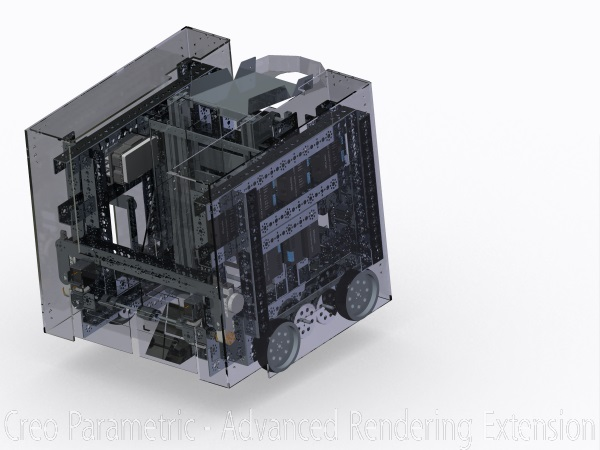
\includegraphics[scale=1]{days/Key_summary/images/A_photo}}
	\end{minipage}
\end{figure}
\begin{figure}[H]
	\begin{minipage}[h]{1\linewidth}
		\center{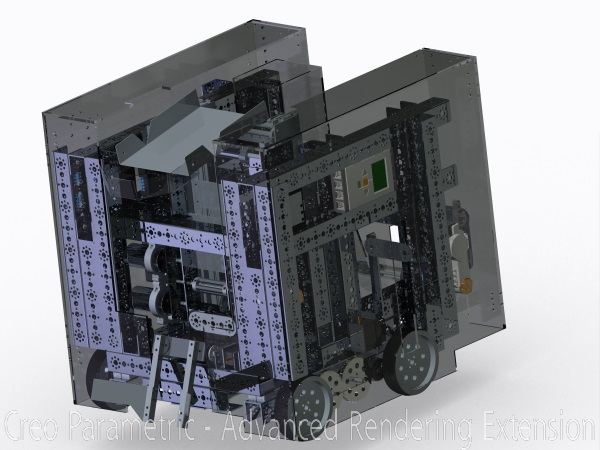
\includegraphics[scale=1]{days/Key_summary/images/A_photo2}}
	\end{minipage}
\end{figure}
\newpage
\subsection{Strategy}
Our strategy is very flexible, so we can adjust to any ally.

\newpage


	
	
\section{Thanks and prospects} 
    We enjoyed working on a custom and non-standard project, which, besides its technical aspect, included working with new people who shared our values of friendship and mutual understanding. 
    
    Our team is planning to continue doing robotics, setting new goals for ourselves in order to improve. This is our first year taking part in FTC and we will participate next year as well. If we don't realize ourselves this year, we'll look at all our mistakes, correct them, and preform a lot better next year.
   
    In any case, we are ready to learn new things, improve ourselves and expand our skills. 
    
    None of us know for sure what we want to do in the future, but we are certain that our experience will be very valuable to us. 
    
    Our thanks go to the company FIRST for organizing this competition, which we are very happy to be participating in. We appreciate this wonderful opportunity to test ourselves and learn something new and wish them success and growth in their future endeavors.
    
    Also we thank our sponsors: company PTC and it's Russian representative "Irisoft" and charitable foundation "Finist" for their support. Also we thank Physics-Mathematics Lyceum 30 and it's director Alexey Tretyakov for providing comfortable conditions for preparation to competition.
   
    
    \begin{center}
      Team PML 30 ${\varphi}$
    \end{center}
    
    \vspace{0.5em}
    
    \begin{figure}[H]
    	\begin{minipage}[h]{0.47\linewidth}
    		\center{
\includegraphics[scale=1]{days/Thanks_for_sponsors/images/01}}
    	\end{minipage}
    	\hfill
    	\begin{minipage}[h]{0.47\linewidth}
    		\center{
\includegraphics[scale=0.2]{days/Thanks_for_sponsors/images/02}}
    	\end{minipage}
    \end{figure}
    
    \vspace{0.5em}
    
    \begin{figure}[H]
    	\begin{minipage}[h]{0.31\linewidth}
    		\center{
\includegraphics[scale=3]{days/Thanks_for_sponsors/images/03}}
    	\end{minipage}
    	\hfill
    	\begin{minipage}[h]{0.31\linewidth}
    		\center{
\includegraphics[scale=0.35]{days/Thanks_for_sponsors/images/05}}
    	\end{minipage}
    	\hfill
    	\begin{minipage}[h]{0.31\linewidth}
    		\center{
\includegraphics[scale=1]{days/Thanks_for_sponsors/images/04}}
    	\end{minipage}
    \end{figure}
    
    \newpage

    %ending:
	%\section{Appendix}



\subsection{Programm}

Program of driver control period and two versions of autonomus period with brief explanations.
\subsubsection{Driver control period}

\subsubsection{Autonomus period from the parking zone}



\subsubsection{Autonomus period from the ramp}


\subsection{Electical scheme}
The final version of the scheme of electrical components of our robot:
\begin{figure}[H]
	\begin{minipage}[h]{1\linewidth}
		\center{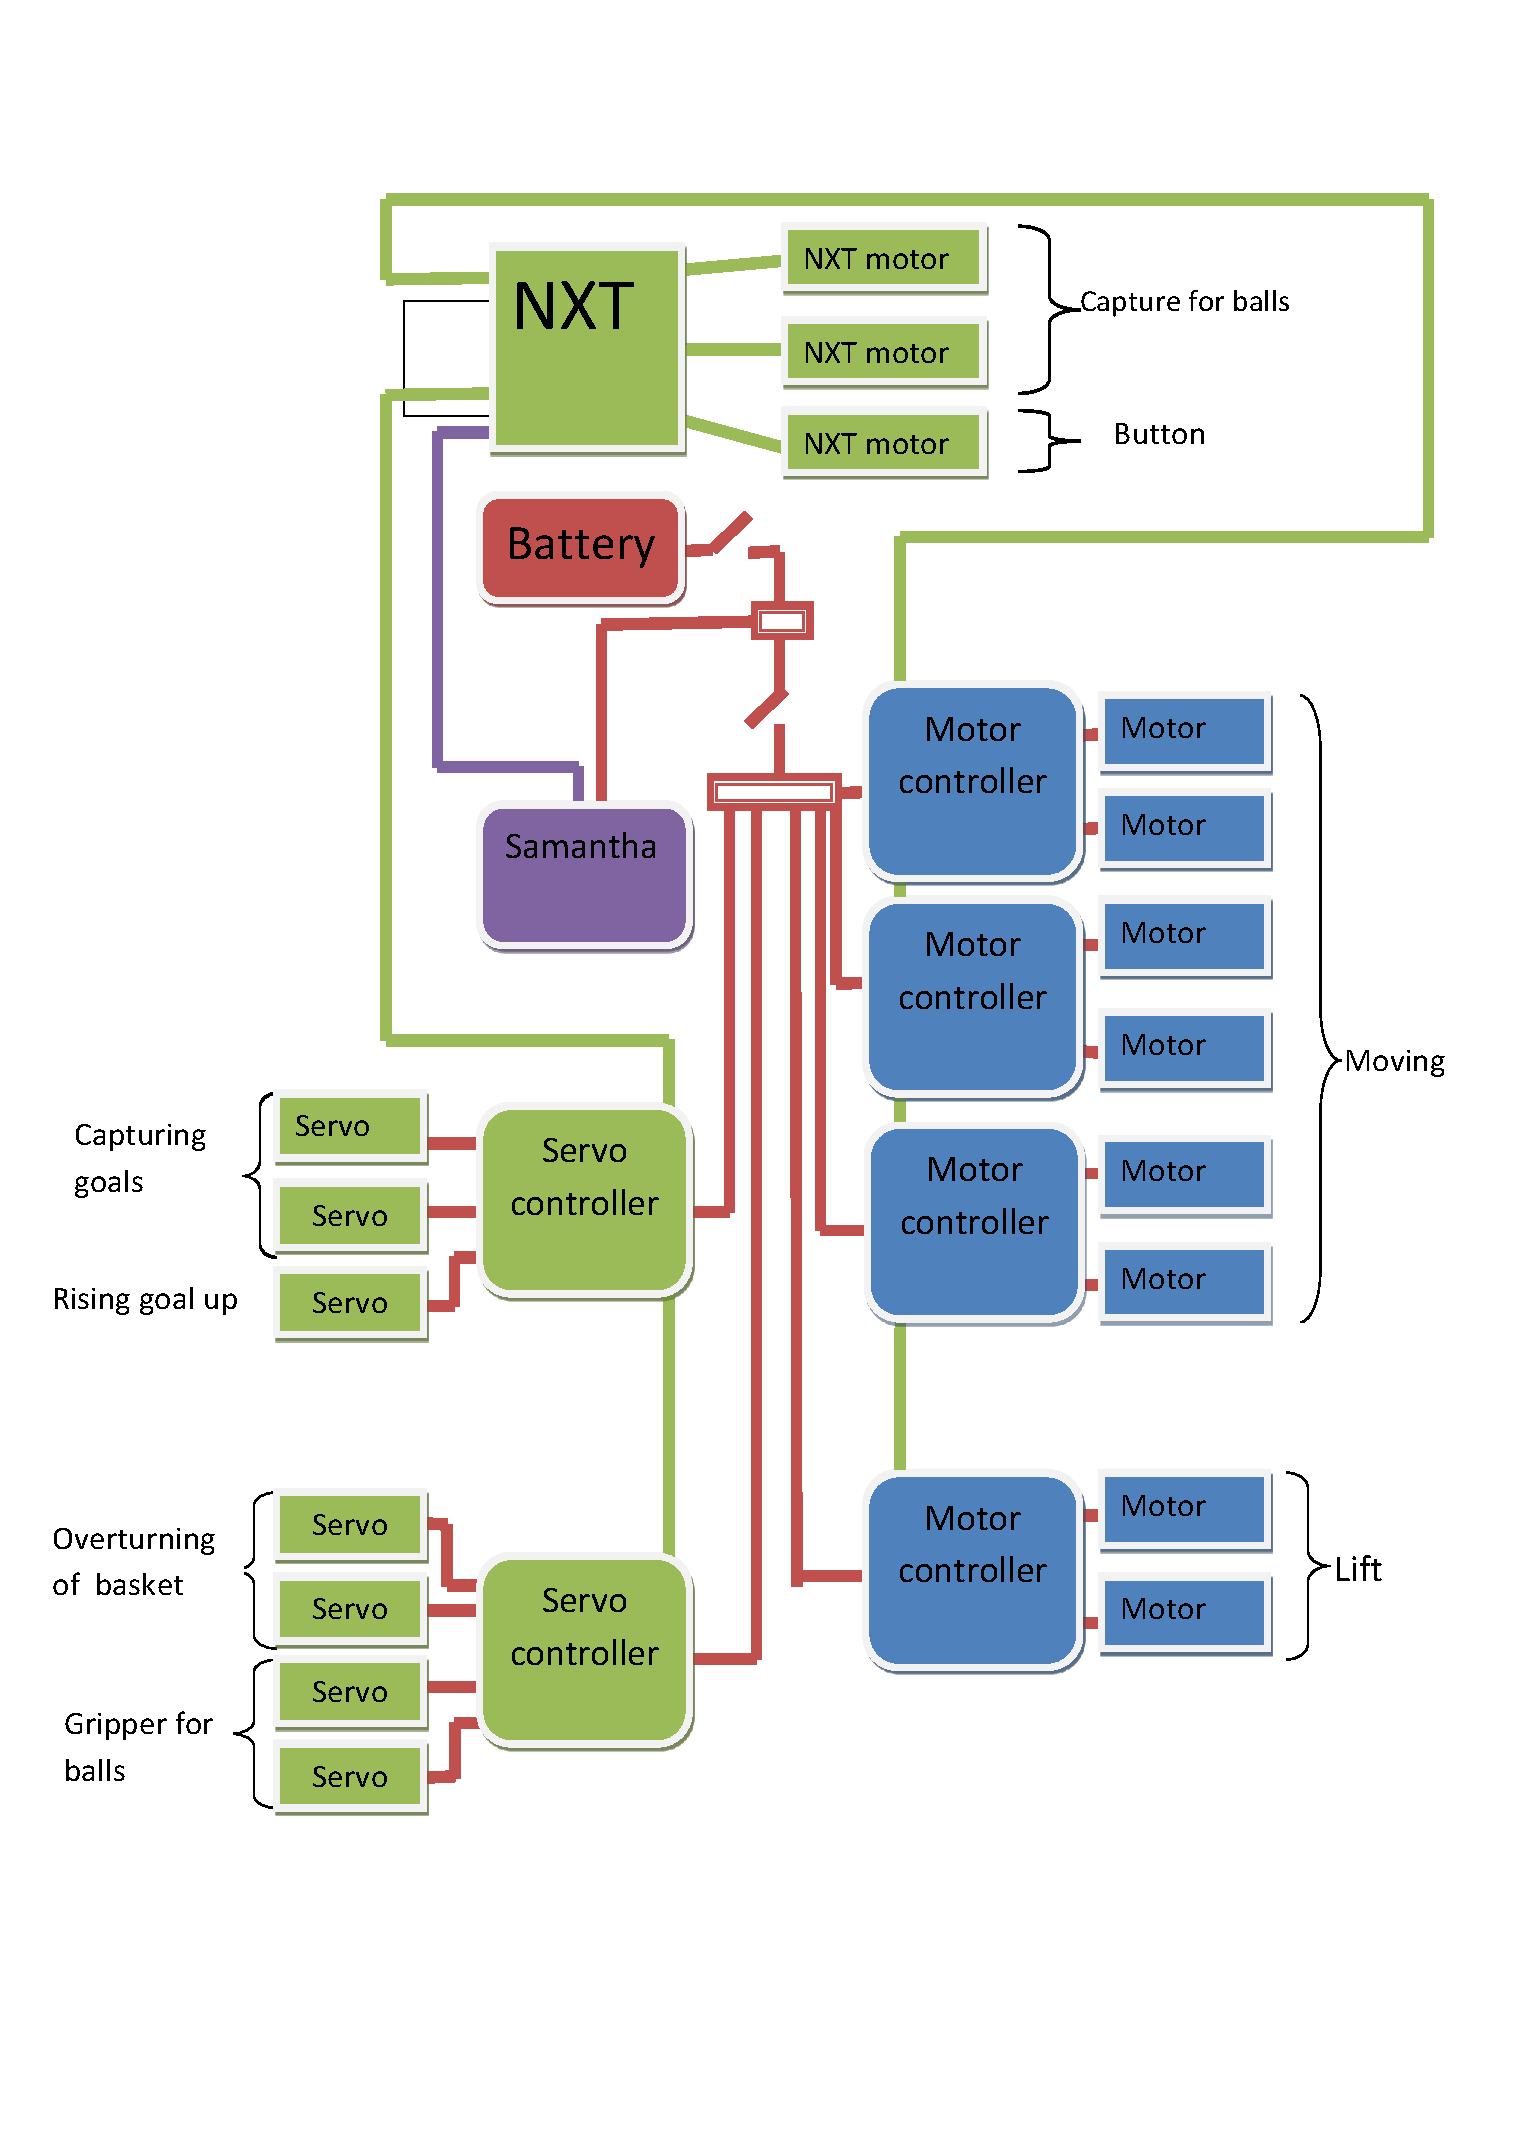
\includegraphics[scale=0.55]{days/Key_summary/images/El-scheme}}
	\end{minipage}
\end{figure}
\fillpage
	%
\subsection{Supplementary materials which were used in the robot's construction}

\begin{enumerate}
	\item Aluminium axis 1m х 8mm. 2 pieces.
	\item Steel axis 3m х 8mm. 1 piece.
	\item Aluminium strip 2m х 50mm х 2mm. 1 piece.
	\item Aluminium strip 1m х 40mm х 3mm. 1 piece.
	\item Aluminium profile 1m х 10mm х 10mm. 1 piece.
	\item Furniture slats 30сm. 2 pieces.
	\item Furniture slats 35сm. 4 pieces.
	\item Belt 2,5m. 1 piece.
	\item Plastic clamps.
	\item Plastic bottle. 1 piece.
	\item List of PET 1 m х 80 cm. 1 piece.
	\item Hot melt adhesive.
	\item Tape.
	\item List of plexiglass 3m x 2m (cut). 1 piece.
\end{enumerate}
\fillpage
\newpage



	
\end{document}
